\chapter{The Temporal Context Model}\label{sec:tcm}
The temporal context model (TCM) was proposed by \textcite{Howard2002} as a model of free recall.
It matched data of immediate, delayed, and continuous distractor recall tasks.
As the distractor task used in the delayed and continuous distractor condition is designed to prevent active rehearsal, this model is likely to address more long-term, synaptic storage as opposed to the short-term OSE model.
Similar to a number of other memory models, the TCM assumes a time varying context signal that items are associated with.
But unlike those other models, this context is based on the items itself rather than being randomly generated.

In particular, items in the TCM are represented as orthogonal vectors $\tcmitem_i$ and the context signal is also a vector $\ctx$.
If we relax the orthogonality constraint on the items to almost (instead of perfectly) orthogonal, we can use Semantic Pointers for these vectors.
To associate items and contexts, two association matrices are used.
The $\mtf$ matrix represents the associations from a context to an item and is constructed as an outer product matrix as
\begin{equation}
    \mtf = \sum_i \tcmitem_i \ctx_i\Tr \text{.}
\end{equation}
Note that the $\mtf$ matrix can be easily updated by adding another item/context outer product.
The $\mft$ matrix is used to retrieve a context vector $\ctxin_i = \mft \tcmitem_i$ to update the current context according to the \emph{evolution equation} (also see \cref{fig:tcm}a)
\begin{equation}
    \ctx_i = \theta_i \ctx_{i-1} + \tcmbeta \ctxin_i\label{eqn:ctx-update}
\end{equation}
where $\tcmbeta$ is a free parameter controlling how fast the context drifts and $0 < \theta_i \leq 1$ is determined to ensure unit length of $\ctx_i$ in each timestep as
\begin{equation}
    \theta_i = \sqrt{1 + \tcmbeta^2 \sbr{\left\langle\ctx_{i-1}, \ctxin_i\right\rangle^2 - 1}} - \tcmbeta \left\langle\ctx_{i-1}, \ctxin_i\right\rangle\text{.}
\end{equation}
In the CUE model, however, $\theta_i$ is fixed to the asymptotic value for $\langle\ctx_{i-1}, \ctxin_i\rangle \rightarrow 0$
\begin{equation}
    \theta_i = \sqrt{1 - \tcmbeta^2}\text{.}
\end{equation}
In the TCM this corresponds to the assumption that item $i$ has not been presented for a sufficiently long time which results in a retrieved context $\ctxin_i$ that is almost orthogonal to the current context.
This change is further motivated by still producing a good match to the data and simplifying the neural implementation as no dynamic scaling of a vector is required.
Such scaling would require a product network for each vector dimension in the NEF\@.
\Cref{eqn:ctx-update} introduces the asymmetric bias to forward recall into the model (\cref{fig:ctxsim}).
While the similarity of contexts $\langle\ctx_i, \ctx_j\rangle$ is symmetric for the lag $j - i$, $\ctxin_i$ is only included in context vectors $\ctx_j$ with $j \geq i$.
\begin{figure}
    \hfill
    \subcaptionbox{}{\begin{tikzpicture}[every path/.style={-Latex}]
        \graph [grow down=1.5cm, branch right=1.5cm] {
            f0/"$\tcmitem_{i-2}$" -> ["$\mft$" anchor=east] cin0/"$\ctxin_{i-2}$" -> ["$\tcmbeta$" anchor=east] c0/"$\ctx_{i-2}$";
            f1/"$\tcmitem_{i-1}$" -> cin1/"$\ctxin_{i-1}$" -> c1/"$\ctx_{i-1}$";
            f2/"$\tcmitem_{i}$" -> cin2/"$\ctxin_{i}$" -> c2/"$\ctx_{i}$";
            start/"$\dots$" [x=-6cm, y=-3cm] -> ["$\theta$" below] c0 -> c1 -> c2 -> end/"$\dots$" [y=-1.5cm];
        };
    \end{tikzpicture}}  % chktex 31
    \hfill
    \subcaptionbox{}{\begin{tikzpicture}[every path/.style={-Latex}]
        \graph [grow down=1.5cm, branch right=1.5cm] {
            start/"$\dots$";
            c0/"$\ctx_i$" -> ["$\mtf$" anchor=east] f0/"$\tcmitemin_i$" -> ["$\mft$" anchor=east] cin0/"$\ctxin_i$";
            c1/"$\ctx_{i+1}$" -> f1/"$\tcmitemin_{i+1}$" -> cin1/"$\ctxin_{i+1}$";
            c2/"$\ctx_{i+2}$" -> f2/"$\tcmitemin_{i+2}$" -> cin2/"$\ctxin_{i+2}$";
            cin0 -> ["$\tcmbeta$" {near end, yshift=-3mm}] c1;
            cin1 -> c2;
            start -> c0 -> ["$\theta$"] c1 -> c2 -> end/"$\dots$";
            cin2 -> end;
        };
    \end{tikzpicture}}  % chktex 31
    \hfill
    \caption{Evolution of the context in the TCM during (a) item presentation and (b) recall.}\label{fig:tcm}
\end{figure}
\begin{figure}
    \centering
    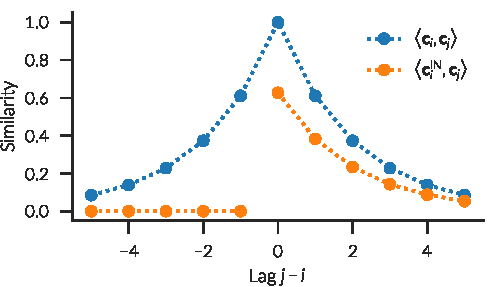
\includegraphics{figures/ctxsim}
    \caption{Similarity of the context to itself $\langle \ctx_i, \ctx_j \rangle$ and to the retrieved context $\langle \ctxin_i, \ctx_j \rangle$ for different lags $j-i$.}\label{fig:ctxsim}
\end{figure}

Finally, the associations from items to context $\mtf$ need to be updated, so that a recalled item can be used to update and partially restore a previous context to retrieve further items.
In the original TCM, this update is given by
\begin{align}
    \mft_{i+1} &= \mft_i \tilde{\mat{P}}_{\tcmitem_i} + a_i \mft_i \mat{P}_{\tcmitem_i} + b_i \ctx_i \tcmitem_i\Tr \\
    a_i &= \gamma b_i \\
    b_i &= \frac{1}{\gamma^2 + 2 \gamma \left\langle\ctxin, \ctx_i\right\rangle + 1}
\end{align}
with projection operators $\mat{P}_{\vc v} = \vc v \vc v\Tr\!/ \norm{\vc v}^2$, $\tilde{\mat{P}}_{\vc v} = \imat - \mat{P}_{\vc v}$, and a free parameter $\gamma$ specifying the relative contribution of previously associated context $\ctxin_i$ and new context $\ctx_i$.
Again, to facilitate the neural implementation, the exact weighting of $\ctxin_i$ and $\ctx_i$ is relaxed while still achieving a good match to data.
Instead of splitting $\mft_i$ into components parallel and orthogonal to $\tcmitem_i$, $\ctx_i\tcmitem_i\Tr$ is added directly into the matrix with a fixed parameter $b$,
\begin{equation}
    \mft_{i+1} = \mft_i + b \ctx_i\tcmitem_i\Tr\text{.}
\end{equation}

Given a context $\ctx$, a mixture of associated items can be recalled as $\tcmitemin = \mtf \ctx$.
To retrieve a single item some form of cleanup has to performed.
Once such a single item has been recalled, the item can be used to recall the associated context as $\mft \tcmitemin$ which in turn can be used to update the current context according to \cref{eqn:ctx-update}.
The updated context allows recalling further items (\cref{fig:tcm}b).

Different cleanup strategies for the recalled item vector can be used.
In the original TCM model, a set of activities $a_i = \tcmitem_i\Tr \tcmitemin$ was obtained and used to make a probabilistic decision according to Luce's choice rule.
The probability of retrieving item $\tcmitem_i$ is given as
\begin{equation}
    P\bigl(\tcmitem_i \bigl|\,\tcmitemin\bigr) = \frac{\exp\!\del{\frac{2a_i}{\tau}}}{\sum_j \exp\!\del{\frac{2a_j}{\tau}}}
\end{equation}
with a parameter $\tau$ that specifies the sensitivity to the activities.

The version of the TCM model presented by \textcite{Sederberg2008}, uses a winner-take-all process based on the leaky, competing accumulator model \parencite{Usher2001}.
In this model, for each possible item a leaky integrator integrates evidence over time.
At the same time, the integrators inhibit each other laterally.
The dynamics can be described by
\begin{equation}
    \vc x_s = \vc x_{s - 1} + \frac{1}{\tau} \del{\vc u - \kappa \vc x_{s - 1} - \lambda \mat L \vc x_{s - 1}} + \vc\eta
\end{equation}
where $\vc u$ is the scaled vector of inputs determined from $\mtf \ctx$ from the current context, $\kappa$ the leak rate, $\lambda$ the lateral inhibition, ${[\mat L]}_{ij} = 1 - \krond_{ij}$ the lateral inhibition matrix, and $\vc\eta$ normal distributed random noise.
This is a more detailed description of how the brain might actually decide for a single item.
However, it is problematic to incorporate within a larger scale neural model under noisy conditions as detailed in \cref{sec:recall}.
For this reason, a different winner-take-all process described in that chapter is used.


\section{Neural context update}\label{sec:ctx-update}

A neural implementation of the TCM needs to implement the updating of $\mft$ and $\mtf$ matrices discussed in \cref{sec:aml}, the recall of items discussed in \cref{sec:recall}, and updating of the context given by \cref{eqn:ctx-update}, discussed in the remainder of this chapter.
Despite being a simple equation, a number of different implementation approaches are potentially viable.
However, only one of these methods was successful in matching the human data when incorporated into the complete model.
It is still instructive to compare these different approaches and consider why they fail.

\subsection{Boundend integrator}
\Cref{eqn:ctx-update} assumes discrete steps, but for a neural implementation a continuous formulation is more natural and given by
\begin{equation}
    \od{\ctx}{t} = (\bar{\rho} - 1) \ctx + \bar{\tcmbeta} \ctxin\,\text{.}
\end{equation}
This equation is easily implemented with a neural integrator for a constant $\bar{\theta}$ and $\bar{\tcmbeta}$.
However, there is no limit on the integration of $\ctxin$ anymore so that the proportion of $\ctxin$ added into $\ctx$ can exceed $\tcmbeta$.
To add at most $\tcmbeta \ctxin$ to the context $\ctx$, we can gate the input to the integrator and add a network computing the dot product between $\ctx$ and $\ctxin$.
After thresholding the dot product at $\tcmbeta$, it can be used to suppress the input by inhibiting the gate ensembles (see \cref{fig:ctx-bounded-integrator}).
Furthermore, in the original TCM $\ctx$ was kept at unit length while the integration has no such bound.
To keep the unit length, we can project $\ctx$ to another population $\ctx_{\downarrow}$ which projects back to the integrator with a transform of $\zeta = -0.1$.
Picking a $\zeta$ closer to zero allows the $\vc c$ vector exceed unit length by a larger amount while the integrator receives input and will increase the time required to settle back to unit length, whereas a large magnitude of $\zeta$ can lead to oscillatory behaviour.
The $\ctx_{\downarrow}$ population needs to be controlled to only provide the inhibitory input to the integrator as long as $\lVert\ctx\rVert > 1$.
This is achieved by decoding the length of $\vc c$ from the integrator and thresholding it at $1$.
As long as the threshold is not exceeded $\ctx_{\downarrow}$ is inhibited.
\begin{figure}
    \centering
    \begin{tikzpicture}[nef]
        \graph {
            in/\ctxin [ext] -!- {
                gate/ [ea] -> ["$\bar{\tcmbeta}$"] integrator/\ctx [ea] -> out/ [ext],
                threshold/ [rect] -!- downscale/$\ctx_{\downarrow}$ [ea] -!- length/ [rect],
                dot [net]
            },
            in -> gate,
            in -> dot -> threshold -> [inhibit, "$\Heavi(x - \tcmbeta)$" {rotate=90}] gate,
            integrator -> dot,
            integrator -> [recurrent, "$\bar{\rho}$" above] integrator,
            integrator -> [bend right] downscale -> [bend right, "$\zeta$" {xshift=-2mm}] integrator,
            integrator -> ["$1 - \norm{\ctx}$" {anchor=south west}] length -> [inhibit] downscale
        };
    \end{tikzpicture}
    \caption{Bounded integrator network}\label{fig:ctx-bounded-integrator}
\end{figure}

To investigate the behaviour of the network, it was fed with new context vectors $\ctxin$ at rate of one vector per second.
These vectors were either orthogonal or had a cosine similarity of \num{0.6} between successive pairs.
\Cref{fig:bounded-integrator} shows the mean similarity of the context vector to itself with given time lag.
For (almost) orthogonal vectors $\ctxin$, the similarity between the context vectors is close under the target.
For non-orthogonal vectors with $\langle\ctxin_i, \ctxin_{i+1}\rangle \approx 0.6$, however, the similarity of the context vectors is by far larger than the target.
This is caused by the input already being similar to the context and thus stopping the update too early.
Note that it is not sufficient to simply adjust $\tcmbeta$ as depending on the similarity of the inputs it needs to either be incremented or decremented.
\begin{figure}
    \centering
    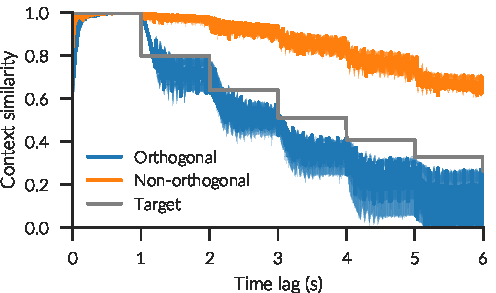
\includegraphics{figures/context-analysis/bounded-integrator}
    \caption[Decay in context similarity with the bounded integrator network]{
        Decay in context similarity with the bounded integrator network given almost orthogonal inputs and inputs with a similarity of approximately \num{0.6}.
        The desired similarity is given by the gray line. Shaded regions indicate \SI{95}{\percent} confidence intervals.}\label{fig:bounded-integrator}
\end{figure}

\subsection{Alternating update of two memories}
With a single integrator, we have to rely on the dot product between the input vector and current context as a measure of $\tcmbeta$.
This dot product is biased in different directions if the input vectors have differing similarities.
To circumvent this, we need to use two gated memory populations that are updated in alternating fashion.
Then the output of the old context and input vector can be combined according to $\theta \ctx + \tcmbeta \ctxin$ and fed into to the memory buffer for the current context.
The completion of that memory update can be detected by the dot product of the updated context and the current context crossing a threshold of one.
Such a network is shown in \cref{fig:ctx-alt-update}.
\begin{figure}
    \centering
    \begin{tikzpicture}[nef, x=2cm, y=2cm]
        \graph [no placement] {
            in/\ctxin [ext, at={(0,0)}] -> ["$\tcmbeta$"] new/ [pnode, at={(1,0)}] -> cgate/ [ea, at={(2, 1)}] -> current/\ctx [ea, at={(3, 1)}] -> oldgate/ [ea, at={(3, -1)}] -> old/$\ctx'$ [ea, at={(2, -1)}] -> ["$\rho$"] new,
            current -> [bend right, "$-1$"] cgate,
            new -> [out=0, in=225] dot [net, at={(4, 1)}], current -> dot [net],
            dot -> rectification/ [rect, at={(4.5, 0.5)}] -> ["$\Heavi(x)$" anchor=west] heavi/ [pnode, at={(4.5, -0.5)}] -> [inhibit, bend left] cgate,
            heavi -> [inhibit] invert/ [ens, at={(4, -1)}] -> [inhibit] oldgate,
            bias/"$1$" [ext, at={(4.5, -1)}] -> invert,
            old -> [bend right, "$-1$" below] oldgate
        };
    \end{tikzpicture}
    \caption{Alternating update of memory buffers}\label{fig:ctx-alt-update}
\end{figure}

Unfortunately, this still does not work for non-orthogonal input vectors (\cref{fig:amb}).
In that case the dot product of the updated context and current context are already quite high and the updated context is not completely loaded into the current memory buffer.
\begin{figure}
    \centering
    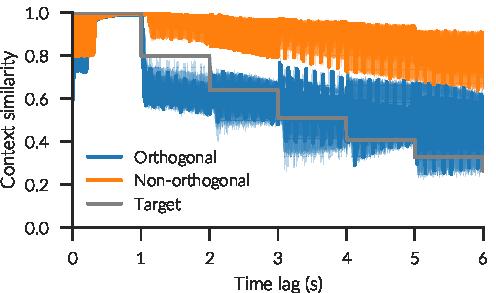
\includegraphics{figures/context-analysis/amb}
    \caption[Decay in context similarity with the alternating update of two memories]{
        Decay in context similarity with the alternating update of two memories given almost orthogonal inputs and inputs with a similarity of approximately \num{0.6}.
        The desired similarity is given by the gray line. Shaded regions indicate \SI{95}{\percent} confidence intervals.}\label{fig:amb}
\end{figure}


\subsection{Externally controlled alternating memory buffers}
All approaches to determine required context updates based on vector similarity will fail because the similarity of $\ctxin_i$ and $\ctx_{i-1}$ is not known beforehand and can vary widely depending on what contexts are recalled.
Thus, for a properly working context update in the TCM model, the update process has to be controlled by an external control signal (see \cref{sec:control}).
% TODO can you say what the content of the control signal is here, so it's 
% clearer what the circuit is being told to do?
If we take the alternating memory buffer network, but control the updating externally (\cref{fig:ctx-ext-ctrl}), it works for both orthogonal and similar input vectors (\cref{fig:ext-amb}).
\begin{figure}
    \centering
    \begin{tikzpicture}[nef, x=2cm, y=2cm]
        \graph [no placement] {
            in/\ctxin [ext, at={(0,0.5)}] -> ["$\tcmbeta$"] new/ [pnode, at={(1,0.5)}] -> cgate/ [ea, at={(2, 1)}] -> current/\ctx [ea, at={(3,1)}] -> oldgate/ [ea, at={(3, -1)}] -> old/$\ctx'$ [ea, at={(2, -1)}] -> ["$\rho$" {very near start, below}] new,
            current -> [bend right, "$-1$"] cgate,
            keep/"keep context" [ext, at={(0,-.5)}] -> ctrl/ [pnode, at={(1,-.5)}] -> [inhibit] cgate,
            ctrl -> ["$-1$" near end] invert/ [pnode, at={(2.5, -0.5)}] -> [inhibit] oldgate,
            bias/$1$ [ext, at={(2.5, 0)}] -> invert,
            old -> [bend right, "$-1$" below] oldgate
        };
    \end{tikzpicture}
    \caption{Alternating update of memory buffers with external control}\label{fig:ctx-ext-ctrl}
\end{figure}
\begin{figure}
    \centering
    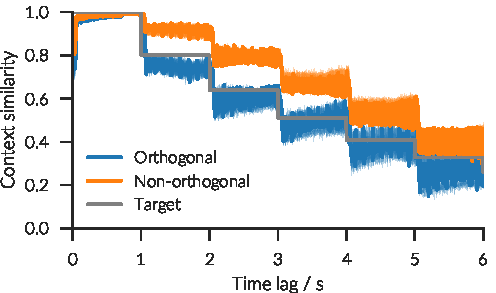
\includegraphics{figures/context-analysis/ext-amb}
    \caption[Decay in context similarity with the alternating update of two memories and external control]{
        Decay in context similarity with the alternating update of two memories and external control given almost orthogonal inputs and inputs with a similarity of approximately \num{0.6}.
        The desired similarity is given by the gray line. Shaded regions indicate \SI{95}{\percent} confidence intervals.}\label{fig:ext-amb}
\end{figure}

This leads to two predictions.
First, the update of the context signal is not directly regulated by the input, but externally controlled.
Second, there are neural populations that start representing the current context in succession.
% TODO I'm not sure what this last bit means (represent in succession?), coudl 
% you add a few sentences to explain the prediction?
